\subsubsection*{Training Insights}
ResNet training came with a lot of randomness over all different models. This is reflected in many trainings that could not perform well at all.
Some runs for example suffered from overfitting (see \autoref{fig:resnet50_bad_training}) while others weren't able to pick up any useful features and validation loss kept on spiking up every other epoch (see \autoref{fig:resnet50_best_history} between epoch 1000 and 1500).

\begin{figure}[H]
\centering
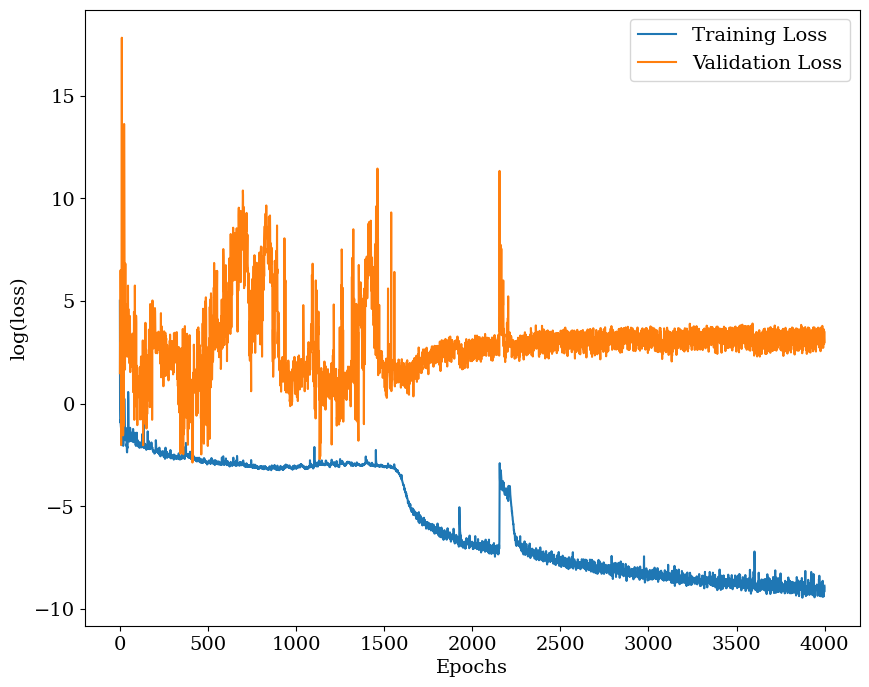
\includegraphics[width=.667\textwidth]{images/Chapter4/ResNet50/res50_bad_history.png}
\caption{ResNet50 with a bad training run. It occasionally reached lower validation loss values but in the end it started to overfit massively after a few thousand epochs of training, indicated by the increase of validation loss and simultaneous decrease of training loss.} 
\label{fig:resnet50_bad_training}
\end{figure}

Many trainings reached good estimations of a galaxy cluster masses relative to its other predictions but under-predicting all values. This is indicated by a smaller $\sigma$ with a high $\mu$ value.

\begin{figure}[H]
\centering
\begin{subfigure}{.46\textwidth}
\centering
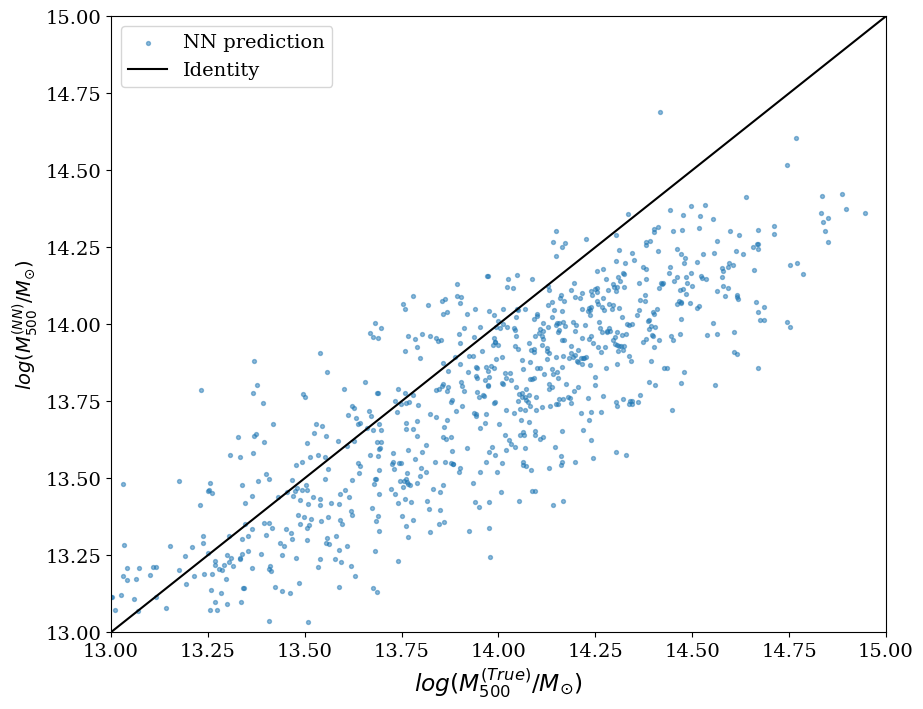
\includegraphics[width=\textwidth]{images/Chapter4/ResNet50/best_but_not_pred.png}
\caption{Predictions from a ResNet50 model with good $\sigma$ but bad $\mu$. The model has difficulties with masses higher than $\log{(M_{500}^{\text{true}}/M_{\odot})} \sim 14$} 
\label{fig:bad_mu}
\end{subfigure}
\hspace{.6em}
\begin{subfigure}{.46\textwidth}
\centering
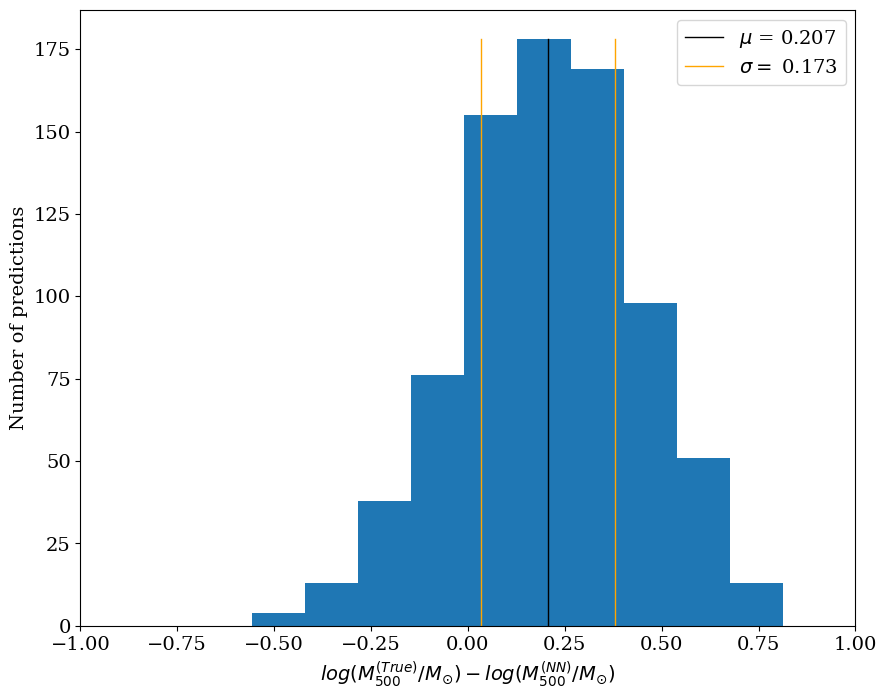
\includegraphics[width=\textwidth]{images/Chapter4/ResNet50/best_but_not.png}
\caption{Histogram of ResNet50 model predictions with good $\sigma$ but bad $\mu$. The whole histogram is shifted towards the right, caused by the positive $\mu$ value.} 
\label{fig:bad_mu_hist}
\end{subfigure}
\caption{A ResNet50 model that was able to get a good sense of the cluster mass in relation to other clusters but under-predicting almost all values, especially at masses higher than $\log{(M_{500}^{\text{true}}/M_{\odot})} \sim 14$.}
\label{fig:bad_mu_comp}
\end{figure}




\subsubsection*{Best Performing Model}
Because of the problems I mentioned before, I did not chose the model with the lowest $\sigma$ on the test set to be the best model because its average mass difference $\mu$ is quite big with $0.18$. Moreover, it had some massive over estimations on the training set. This makes the $\sigma$ and $\mu$ explode on this set. Because of that I went with a training that had a higher $\sigma$ on the test set with $\sigma = 0.185$ (rather than the $0.171$) but was more evenly spread around the identity with a $\mu$ of $0.035$.

\begin{figure}[H]
\centering
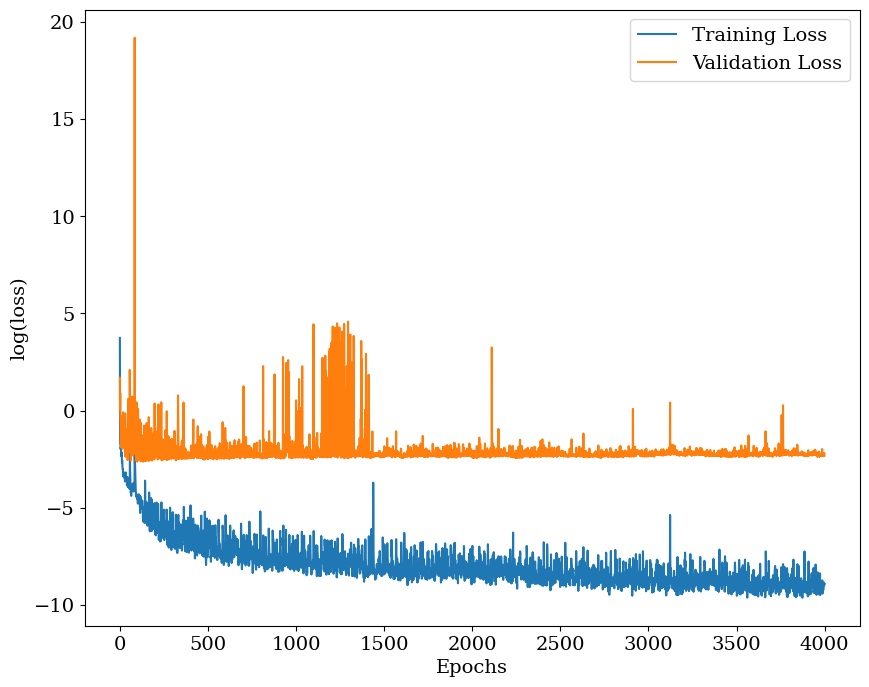
\includegraphics[width=.667\textwidth]{images/Chapter4/ResNet50/res50_best_history.png}
\caption{Best performing ResNet50 model after ten training runs. After more spikes in validation loss at the beginning, as the training loss kept on decreasing the validation loss settled at around $0.01$. A slightly lower validation loss after around $200$ epochs might be an indication for overfitting.} 
\label{fig:resnet50_best_history}
\end{figure}


\begin{figure}[H]
\centering
\begin{subfigure}{.46\textwidth}
  \centering
  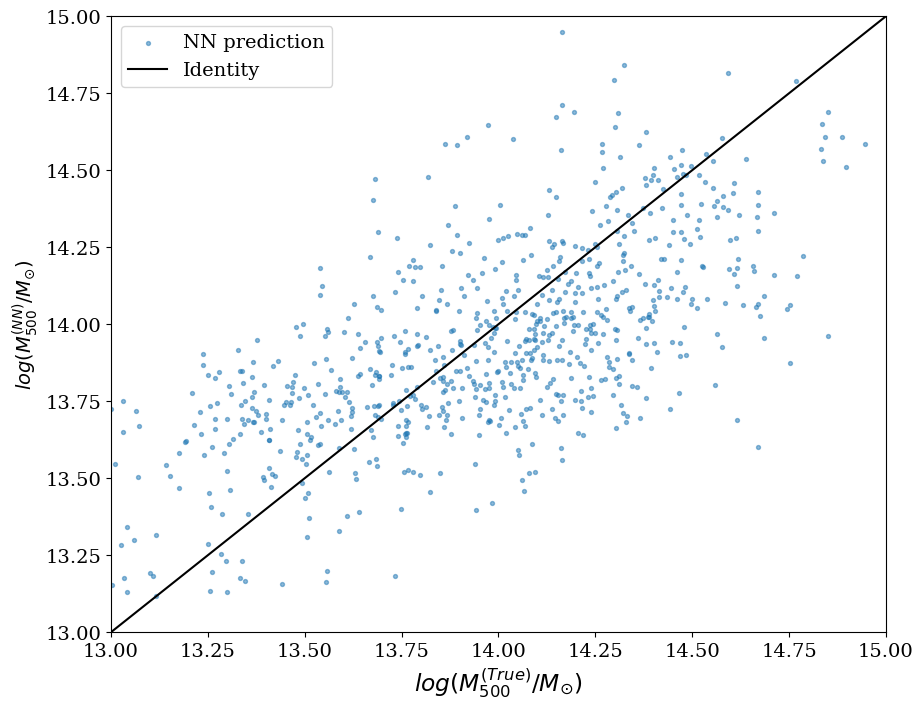
\includegraphics[width=\linewidth]{images/Chapter4/ResNet50/res50_best_test.png}
  \caption{Model predictions on the test set.}
  \label{fig:best_perf_resnet50_a}
\end{subfigure}%
\hspace{.6em}
\begin{subfigure}{.46\textwidth}
  \centering
  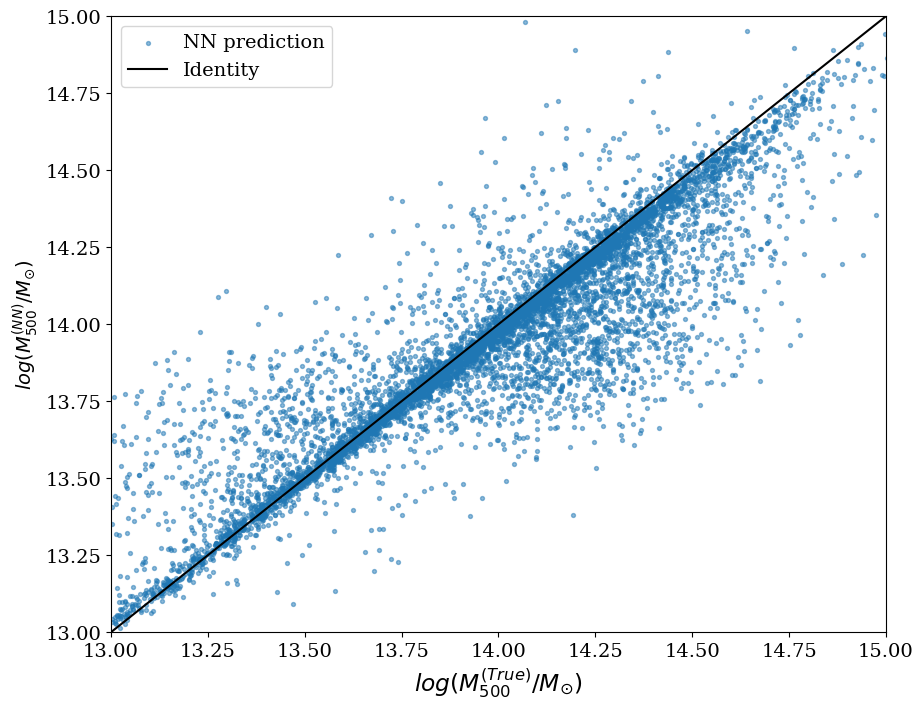
\includegraphics[width=\linewidth]{images/Chapter4/ResNet50/res50_best_train.png}
  \caption{Model predictions on the training set.}
  \label{fig:best_perf_resnet50_b}
\end{subfigure}
\begin{subfigure}{.46\textwidth}
  \centering
  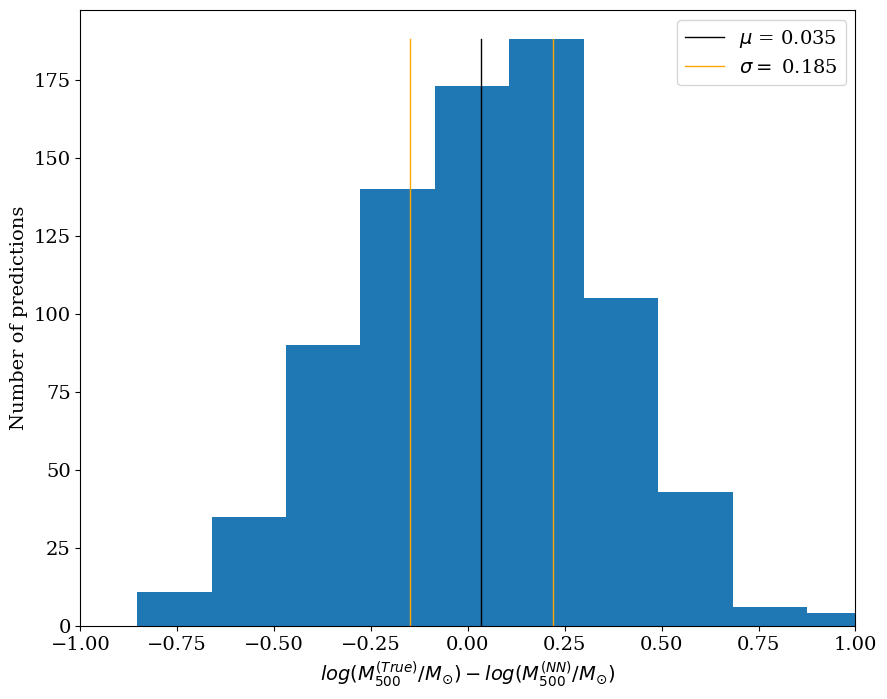
\includegraphics[width=\linewidth]{images/Chapter4/ResNet50/res50_best_test_hist.png}
  \caption{Histogram of model predictions on the test set.}
  \label{fig:best_perf_resnet50_c}
\end{subfigure}%
\hspace{.6em}
\begin{subfigure}{.46\textwidth}
  \centering
  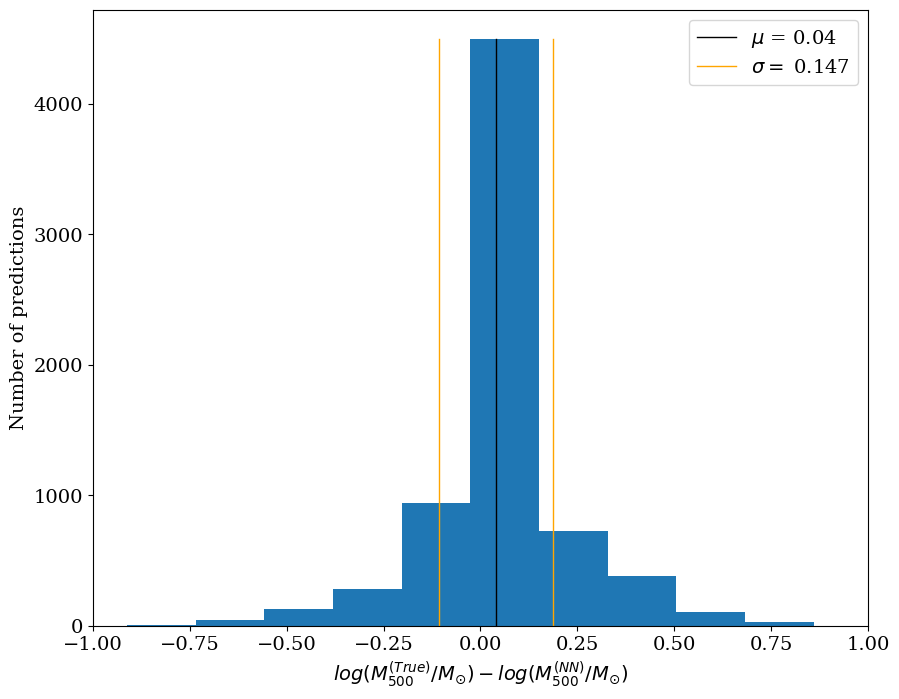
\includegraphics[width=\linewidth]{images/Chapter4/ResNet50/res50_best_train_hist.png}
  \caption{Histogram of model predictions on the training set.}
  \label{fig:best_perf_resnet50_d}
\end{subfigure}
\caption{Prediction analysis for ResNet50 model. Predictions on the training set indicate overfitting.} 
\label{fig:best_perf_resnet50}
\end{figure}

On the test set the predictions are too high for smaller galaxy clusters, and too low for bigger galaxy clusters. All in all they are widely spread and are considerably worse than the basic CNN's best model.
The predictions on the training set look very similar to the predictions received in \autoref{fig:overf_comp_train}, indicating overfitting. This was also seen in the training history (see \autoref{fig:resnet50_best_history}), where the validation loss had its minimum after $200$ epochs. This shows that the model might be capable of accurate mass estimations after optimization. To improve the ResNet50 model, adjustments in training speed might yield better results.